\section{Functional Verification Methodology}
\label{sec:sbsmethod}
We run SBS on a set of building sensor traces; each containing hundred sensors reporting data flows over 18 weeks from two separate buildings with fundamentally different infrastructures.  
We demonstrate that, in many cases, SBS uncovers misbehavior corresponding to inefficient device usage that leads to energy waste.  
The average waste uncovered is as high as 2500~kWh per device. 

We validate the effectiveness of our approach using 10 weeks of data from a modern Japanese building containing 135 sensors and 
8 weeks of data from an older American building containing 70 sensors.
These experiments highlight the effectiveness of SBS to uncover device relationships in a large deployment of 135 sensors.
Furthermore, we inspect the SBS results and show that the reported alarms correspond to significant opportunities to save energy.
The major anomaly reported in the American building lasts 18 days and accounts for a waste of 2500 kWh. % for a single device whereas the building average power consumption is 600 kW per hour.
% SBS also reported numerous smaller anomalies that are hidden in the building's overall consumption, thus, difficult for building operators to identify without the proposed method.
SBS also reports numerous small anomalies, hidden deep within the building's overall consumption data.  Such errors are very difficult to find
without SBS.
% \subsection{Problem description}
% \subsection{Dominant patterns}

\begin{figure}
\begin{center}
\includegraphics[width=.5\textwidth]{figs/heatMap_raw_201106-eps-converted-to.pdf}
\caption{Correlation coefficients of the raw traces from the Building 1 dataset (Section \ref{data:engbldg2}).
The matrix is ordered such as the devices serving same/adjacent rooms are nearby in the matrix.}
\label{fig:heatmap:raw}
\end{center}
\end{figure}

%The first step of the proposed approach is to uncover from the raw data the devices that are used all together.
The primary objective of SBS is to determine \emph{how} device usage patterns are correlated across all pairs of sensors and 
discover when these relationships change.  
%The basic tool that allows us to compare device energy consumption is the correlation coefficient.
%Classical approaches would run correlation analyses across pairs of power-draw signals between distinct devices, summarized by a correlation coefficient.
The naive approach is to run correlation analysis on pairs of sensor traces, recording their correlation coefficients over time and 
examining when there is a statistically-significant deviation from the norm.  
However, this approach does not yield any useful information when applied to \emph{raw data traces}.
%However, during our experiments we found that it provides poor help when it is directly applied to the raw signals.
For example, the two raw signals shown in Figure~\ref{fig:diagram1} are from two independent HVAC systems,
 serving different rooms on different floors.
Since each space is independently controlled, we expect their power-draw signals to be uncorrelated (or at least distinguishable 
from other signal pairs).  However, their correlation coefficient ($0.57$), is not particularly informative -- it is statistically
similar to the correlation between itself and other signals in the trace.  
% however, their correlation coefficient (i.e. $0.5675$) indicates the opposite.
%Another example, with 135 devices, is depicted in Figure \ref{fig:heatmap:raw}.

% Another example, depicted in Figure \ref{fig:heatmap:raw}, shows a correlation matrix with 135 distinct locations, each containing a number of devices.  
Using a larger set of devices, Figure \ref{fig:heatmap:raw} shows a correlation matrix with 135 distinct lighting and HVAC systems serving numerous rooms in a building (described later on in Section \ref{data:engbldg2}).
The indices are selected such that their index-difference is indicative of their relative spatial proximity.  
For example, a device in location 1 is closer in the building to a device in location 2 than it is to 
a device in location 135. 
% We do not account for obstructions between them, such as walls.  %?
The color of the cell is the average pairwise correlation coefficient for devices in the row-column index.  The higher the value, the lighter the color.
%the devices serving the same (or adjacent) room are close
%to one another in the matrix.  
Devices serving the same room are along the diagonal.  Because these devices are used simultaneously, we expect
high average correlation scores, lighter shades, along the diagonal figure.
%and because they are used simultaneously by the room users we expect them to feature the highest correlation scores.
However, we observe no such pattern.  %structure is unseen in the Figure.  
Most of the signals are correlated with all the others and we see no discernible structure.
% thus this metric prevents us from finding devices that are used in concert.

\begin{figure}[t!]
\begin{center}
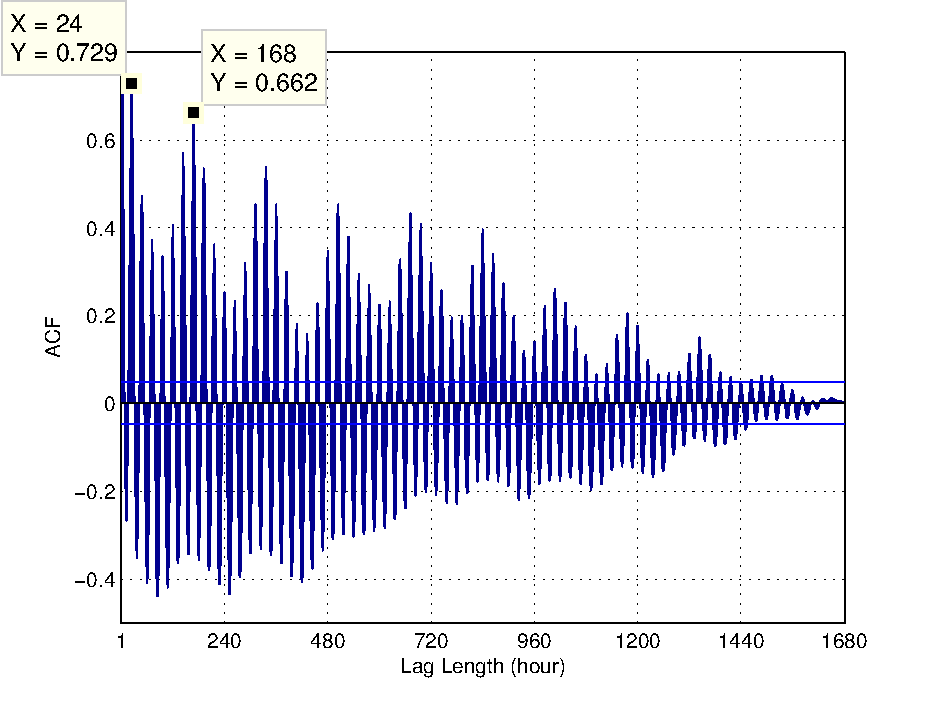
\includegraphics[width=.5\textwidth]{figs/acf_101A1_GHP-eps-converted-to.pdf}
\caption{Auto-correlation of a usual signal from the Building 1 dataset.
The signal features daily and weekly patterns (resp. $x=24$ and $x=168$).}
\label{fig:autocorr}
\end{center}
\end{figure}

An explanation for this is that the daily occupant usage patterns %office hours, 
drive these results.
Figure \ref{fig:diagram1} demonstrates this more clearly.  It shows two 1-week raw signals traces which feature the same 
diurnal pattern.  
This trend is present in almost every sensor trace, and, it hides 
the smaller fluctuations providing more specific patterns driven by local occupant activity.  Upon deeper inspection, we uncovered several
 dominant patterns, common among energy-consuming devices in buildings~\cite{wrinch:pes2012}.  Figure~\ref{fig:autocorr} depicts the 
 auto-correlation of a usual electric power signal for a device.  The two highest values in the figure correspond to a lag of 24 hours and 168 hours (one week).  
 Therefore, the signal has some periodicity and similar (though not equal) values are seen at daily and weekly time scales.
The daily pattern is due to daily office hours and the weekly pattern corresponds to weekdays and weekends.  
%Indeed, thorough inspection of the data reveals that the 
Correlation analysis on \emph{raw} signals cannot be used to determine meaningful 
inter-device relationships because periodic components act as non-stationary trends for high-frequency phenomenon, 
 making the correlation function irrelevant.  %metric is insufficient with raw signals containing the same dominant pattern.
Such trends must be removed in order to make meaningful progress towards our aforementioned goals.  

In the next section we describe SBS.  
We discuss \emph{strip and bind} in section~\ref{methodo:est}, which addresses de-trending and
relationship-discovery.  Then, we describe how we \emph{search} for changes in usage patterns, 
in section~\ref{methodo:ano}, to identify potential savings opportunities.

%One of the major challenges in this work is to discard these patterns and uncover devices intrinsic relationships.
% This difficulty is overcome by the first part of the method (Strip and Bind) presented in Section \ref{methodo:est}.
% Then, the second part of the method (Search) monitors over time the devices relationships and detect abnormal device behavior changes (Section \ref{methodo:ano}).


% \subsection{Methodology}\label{methodo}

\subsubsection{Strip and Bind} \label{methodo:est}

\begin{figure}[t!]
\begin{center}
 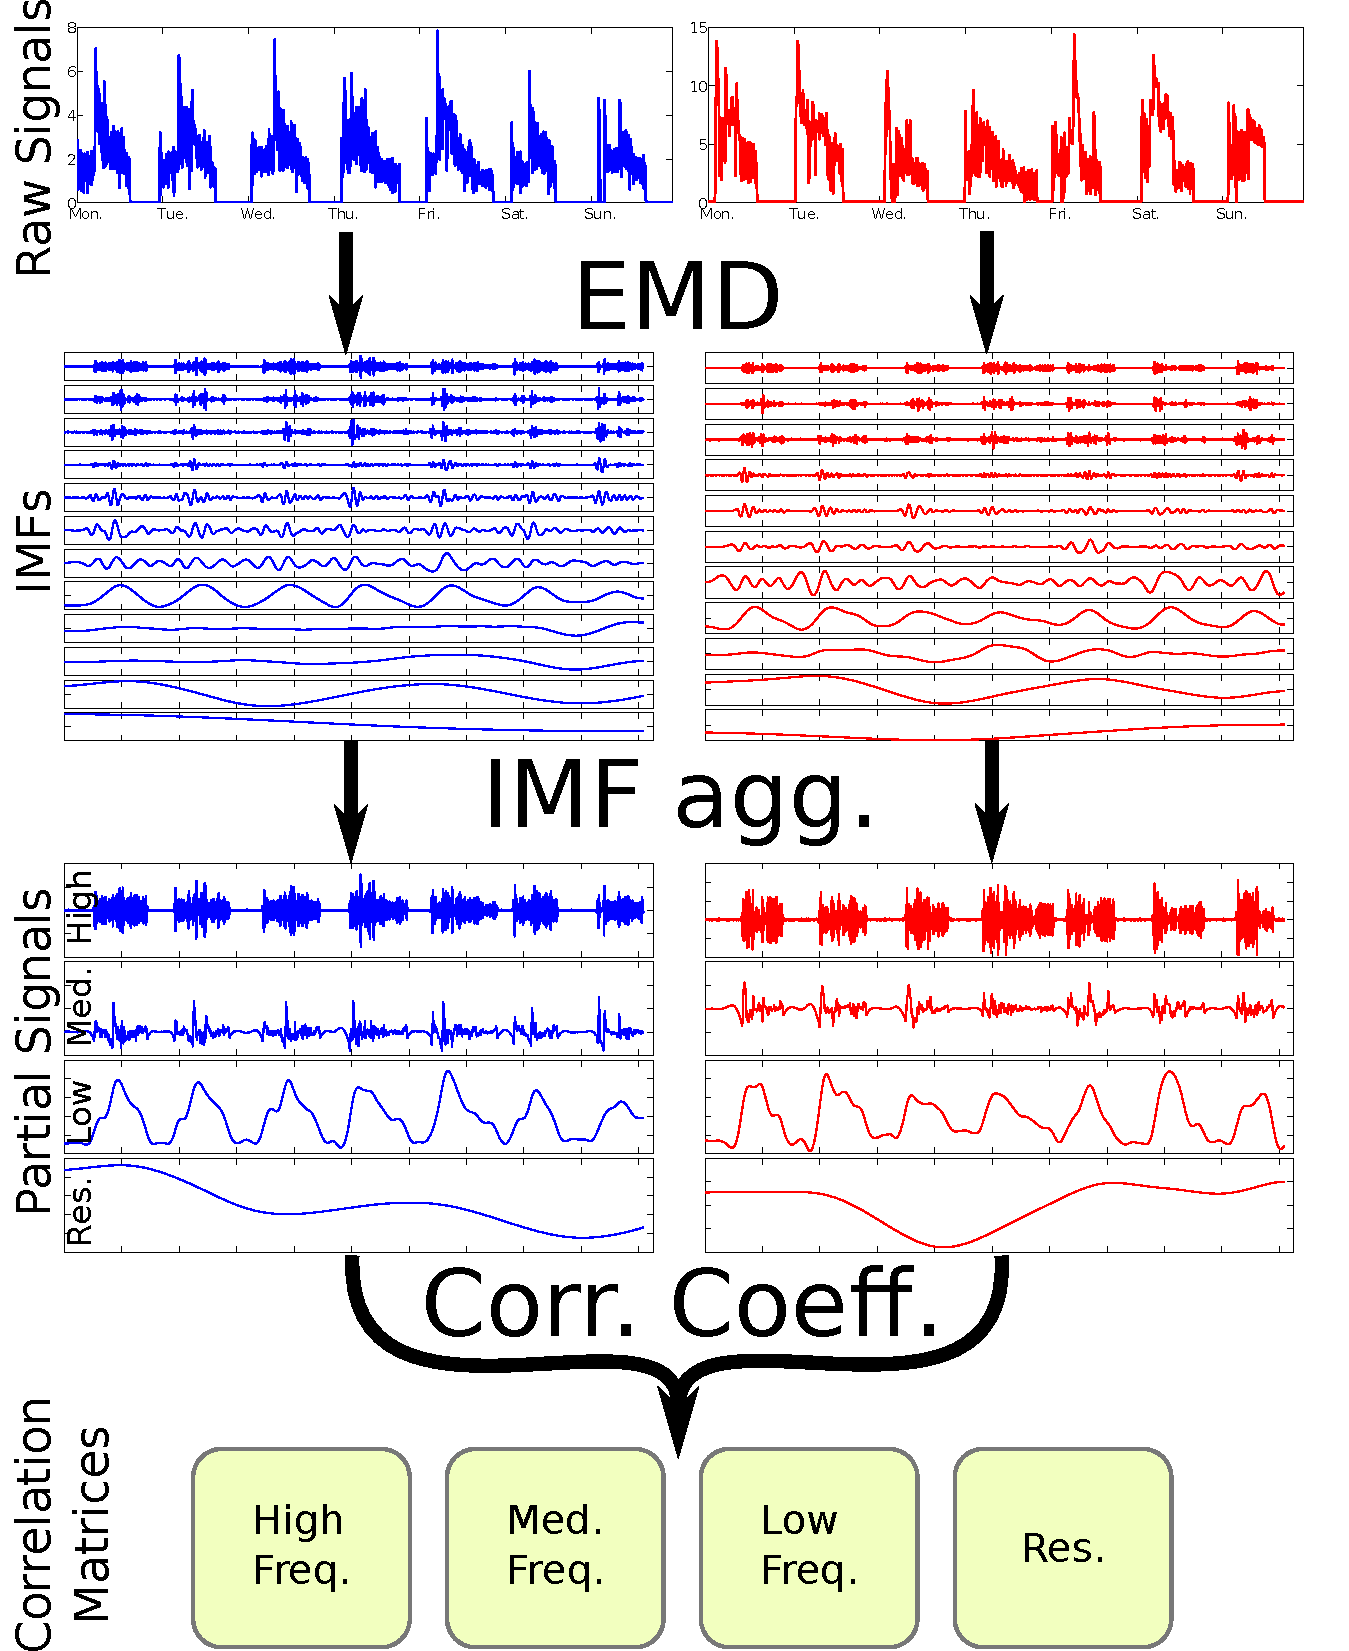
\includegraphics[width=.5\textwidth]{figs/estimator.pdf}
 \caption{\emph{Strip and Bind} using two raw signals standing for one week of data from two different HVACs. (1)~Decomposition of the signals in IMFs using EMD (top to bottom: $c_1$ to $c_n$); (2)~aggregation of the IMFs based on their time scale; (3)~comparison of the partial signals (aggregated IMFs) using correlation coefficient.}
 \label{fig:diagram1}
 \end{center}
\end{figure}

%As shown in the previous section, discovering the devices that are used in concert is particularly difficult.
Discovering devices that are used in concert is non-trivial.  
SBS decomposes each signal into an additive set of components, called Intrinsic Mode Functions (IMF), 
that reveals the signal patterns at different frequency bands.  IMFs are obtained using 
%that reveal the signal structures at different time scales.
Empirical Mode Decomposition (see Figure~\ref{fig:diagram1} and Section~\ref{emd}).
%Then, we filter out the IMFs that interfere with our goal and keep only those standing for time scales shorter than the unwanted daily pattern.
%We then remov out IMFs with time scales 
We only consider IMFs with time scales shorter than a day, since we are interested in capturing short-scale usage patterns.
Consequently, SBS aggregates the IMFs that fall into this specific time scale (see \emph{IMF agg.} in Figure \ref{fig:diagram1}).
%The resulting partial signals of different devices are compared pairwise to identify the devices intrinsic relationships (see \emph{Corr. Coeff.} in Figure\ref{fig:diagram1}). 
The resulting partial signals of different device power traces are compared, pairwise, to identify the devices that show un/correlated usage patterns (see \emph{Corr. Coeff.} in Figure~\ref{fig:diagram1}).


% These intrinsic relations are uncovered by comparing the sensors data at certain meaningful frequency bands.
% Namely, looking at high frequency allows to compare short-term variations representing the instantaneous devices change of state, however, the low frequency highlights long-term fluctuations revealing long devices usage pattern.
% 
% ..... the similarity estimators analyzes the readings from several sensors and reports scores standing for the similarity of the sensors at different frequency bands.
% First, the similarity estimator takes advantage of EMD to decompose the sensors signals into a set of components called intrinsic mode functions (IMFs).
% Second, it constructs band-limited signals by aggregating the IMFs whose mean frequencies fall in a certain frequency band.
% Thereby the pairwise comparison of band-limited signals provides the sensors correlations at different frequency bands. 
% 
% The advantages of the proposed intrinsic-correlation estimator are adaptive approach, ... 

% These two steps are described by the two following sections.



The IMFs are clustered using four time scale ranges: 
\begin{itemize}
 \item The \emph{high frequencies} are all the IMFs with a time scale lower than 20 minutes. These IMFs capture the noise.
 \item The \emph{medium frequencies} are all the IMFs with a time scale between 20 minutes and 6 hours. These IMFs convey the detailed devices usage.
 \item The \emph{low frequencies} are all the IMFs with a time scale between 6 hours and 6 days. These IMFs represent daily device patterns.
 \item The \emph{residual data} is all data with a time scale higher than 6 days. This is mainly residual data obtained after applying EMD.  Also, it highlights the main device trend.
\end{itemize}

These time scale ranges are chosen based on our experiments and goal.
The 20-minute boundary relies on the sampling period of our dataset (5 minutes) and permits us to capture IMFs with really short periods.
The 6-hour boundary allows us to analyze all patterns that have a period shorter than the usual office hours.
The 6-day boundary allows us to capture daily patterns and weekday patterns.

Aggregating IMFs, within each time scale range, results in 4 partial signals representing different characteristics of the device's
 energy consumption (see \emph{Partial Signals} in Figure~\ref{fig:diagram1}).
We do a pairwise device trace comparison, calculating the correlation coefficient of their partial signals.
In the example shown in Figure~\ref{fig:diagram1}, the correlation coefficient of the raw signals suggests that they are highly correlated ($0.57$). 
However, the comparison of the corresponding \emph{partial signals} provides new insights;
the two devices are poorly correlated at high and medium frequencies (respectively $-0.01$ and $-0.04$) but highly correlated at low frequencies ($0.79$) meaning that these devices are not ``intrinsically'' correlated.  They only share a similar daily pattern.

All the devices are compared pairwise at the four different time scale ranges.
Consequently, we obtain four correlation matrices that convey device similarities at different time scales.
Each line of these matrices (or column, since the matrices are symmetric) reveals the behavior of a device -- its relationships with the 
other devices at a particular time scale.
The matrices form the basis for tracking the behavior of devices and to search for misbehavior.


\subsection{Search}\label{methodo:ano}
\emph{Search} aims at identifying misbehaving devices in an unsupervised manner.
Device behavior is monitored via the correlation matrices presented in the previous section.
Using numerous observations SBS computes a specific reference that exhibits the normal inter-device usage pattern.
Then, SBS compares the computed reference with the current data and reports devices that deviate from their usual 
behavior.

\subsection{Reference Matrix}
We define four reference matrices, which capture normal device behavior at the four time scale ranges defined in 
Section~\ref{methodo:corr}.
The references are computed as follows: (1) we retrieve the correlation matrices for $n$ consecutive time bins. (2) For each pair of devices we compute the median correlation 
over the $n$ time bins and obtain a matrix of the median device correlations.

Formally, for each time scale range the computed reference matrix for $d$ devices and $n$ time bins is:
\[R_{i,j} =  \median(C^1_{i,j},...,C^n_{i,j})\]
where $i$ and $j$ ranges in $[1,d]$.

% Assuming that device-usage predominantly behaves normally and the anomalies are exceptional 
% events, the reference matrices exhibit the normal device behaviors.
% Our model assumes anomalies are rare and the majority of the data is normal.
% This is a common assumption in unsupervised anomaly detection.
Because anomalies are rare by definition, we assume the data used to construct the reference matrix
is an accurate sample of the population; it is unbiased and accurately captures the range of normal behavior.
% We assume that normal behavior is not truly anomalous.
Abnormal correlation values, that could appear during model construction, %in the analyzed time bins 
are ignored by the median operator thanks to its robustness to outlier (50\% breakdown point).  
However, if that assumption does not hold (more than 50\% of the data is anomalous), our model will flag the opposite -- labeling abnormal as normal and vice-versa.
From close inspection of our data, we believe our primary assumption is sound.
% Normal behavior occurs most frequently, therefore detected anomalies should be meaningful.



\subsection{Behavior change}
% SBS consists in identifying the devices that significantly deviate from their normal behaviors as defined in the reference matrices.
% Consequently, 
We compare each device behavior, for all time bins, to the one provided by the reference matrix.  
Consider the correlation matrix $C^t$ obtained from the data for time bin $t$ ($1 \leq t \leq n$).  
Vector $C^t_{i,*}$ is the behavior of the $i^{th}$ device for this time bin.
Its normal behavior is given by the corresponding vector in the reference matrix $R_{i,*}$.
We measure the device behavior change at the time bin $t$ with the following Minkowski weighted distance:
\[ l^t_{i} = \left(\sum_{j=1}^d  w_{ij}\left(C^t_{i,j} - R_{i,j}\right)^p\right)^{1/p} \]
where $d$ is the number of devices and $w_{ij}$ is:
\[ w_{ij} = \frac{R_{i,j}}{\sum_{k=1}^d R_{i,k}}. \]
The weight $w$ enables us to highlight the relationship changes between the device $i$ and those highly correlated to it in the reference matrix.
In other words, our definition of behavior change is mainly driven by the relationship among devices that are usually used in concert.
We also set $p=4$ in order to inhibit small differences between $C^t_{i,j}$ and $R_{i,j}$ but emphasize the important ones.

By monitoring this quantity over several time bins the abnormal device behaviors are easily identified as the outlier values.
In order to identify these outlier values we implement a robust detector based on median absolute deviation (MAD), a dispersion measure commonly used in anomaly detection \cite{huber:wiley2009,chan:springer2005}.
It is a measure that robustly estimates the variability of the data by computing the median of the absolute deviations from the median of the data.
 Let $l_{i} = [l_i^1,...,l_i^n]$ be a vector representing the behavior changes of device $i$ over $n$ time bins, then its MAD value is defined as:
\[ \mad_i = b \median(\lvert l_{i} - \median(l_{i})\rvert)\]
where the constant $b$ is usually set to $1.4826$ for consistency with the usual parameter $\sigma$ for Gaussian distributions.
Consequently, we define anomalous behavior, for device $i$ at time $t$, such that the following equation is satisfied:%of the device $i$ at the time bin $t$ that satisfies the following equation:
\[l^t_{i} > \median(l_{i}) + \tau  \mad_i\]
Note, $\tau$ is a parameter that permits to make SBS more or less sensitive.

The final output of SBS is a list of alarms in the form $(t,i)$ meaning that the device $i$ has abnormal behavior at the time bin $t$.
The priority of the alarms in this list is selected by the building administrator by tuning the parameter $\tau$.





We evaluate SBS using data collected from buildings in two different geographic locations.  
One is a new building on main campus of the University of Tokyo and the other is an older building at 
the University of California, Berkeley.

Data pre-processing is not generally required for the proposed approach.  
Nevertheless, we observe in a few exceptional cases that sensors reporting excessively high values (i.e. values higher than the device actual capacity) that  greatly alter the performance of SBS by inducing a large bias in the computation of the correlation coefficient.
Therefore, we remove values that are higher than the maximum capacity of the devices, from the raw data.




The Todai dataset we use contains 10 weeks of data starting from June 27, 2011 and ending on September 5, 2011.
This period of time is particularly interesting for two reasons: 1) in this region, the summer is the most energy-demanding 
season and 2) the building manager actively works to curtail energy usage as much as possible due to the 
Tohoku earthquake and Fukushima nuclear accident.

Furthermore, this dataset is a valuable ground truth to evaluate the Strip and Bind portions of SBS.
Since the light and HVAC of the rooms are directly controlled by the room's occupants, we expect SBS to uncover verifiable devices 
relationships.  


The Cory Hall dataset we use consists of 8 weeks of energy consumption traces measured by 70 sensors starting on April $5^{th}$, 2011.
In contrast to the other dataset, a variety of devices are monitored, including, electric receptacles on certain floors, most of the HVAC components, 
 power panels and whole-building consumption.

These two building infrastructures are fundamentally different.  
This enables us to evaluate the practical efficacy of the proposed, unsupervised method in two very different environments.


\begin{figure*}[t!]
% \subfloat[Raw signals]{\includegraphics[width=.48\textwidth]{img/heatMap_raw_201106-eps-converted-to.pdf}}\\
\subfloat[High Frequencies\label{fig:heatmap:high}]{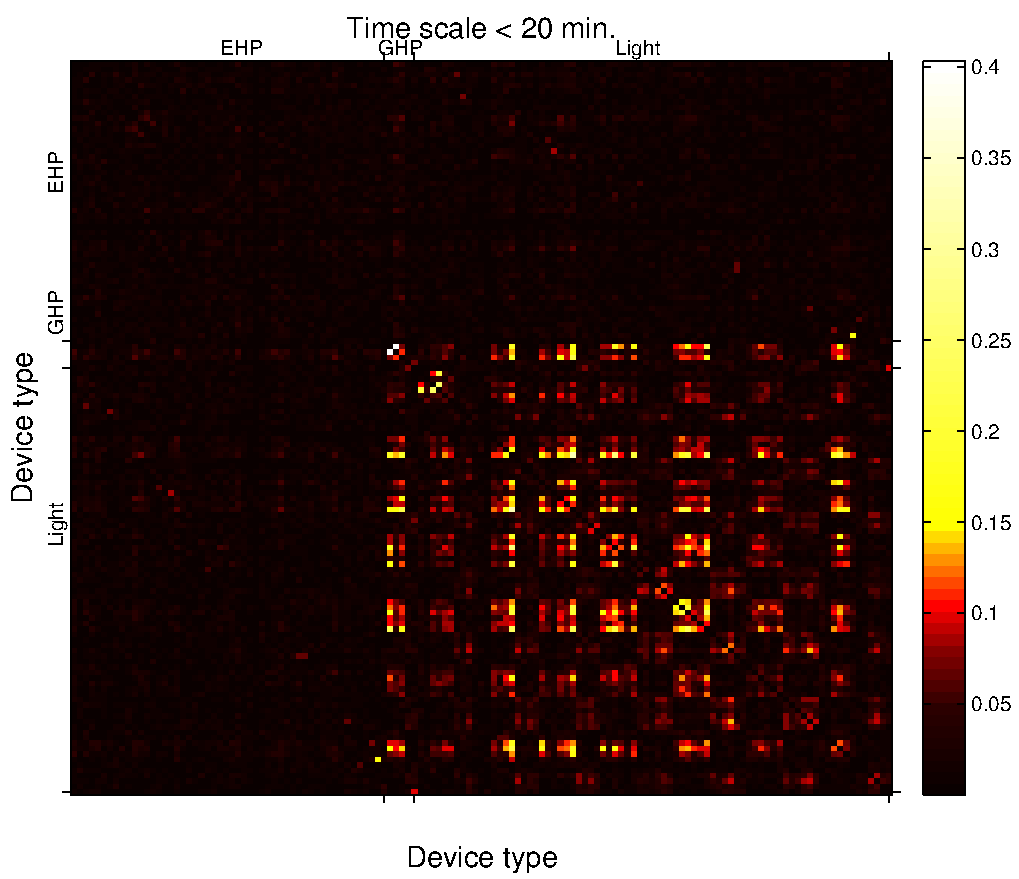
\includegraphics[width=.48\textwidth]{figs/heatMap_1_201106-eps-converted-to.pdf}}\hfill
\subfloat[Medium Frequencies\label{fig:heatmap:med}]{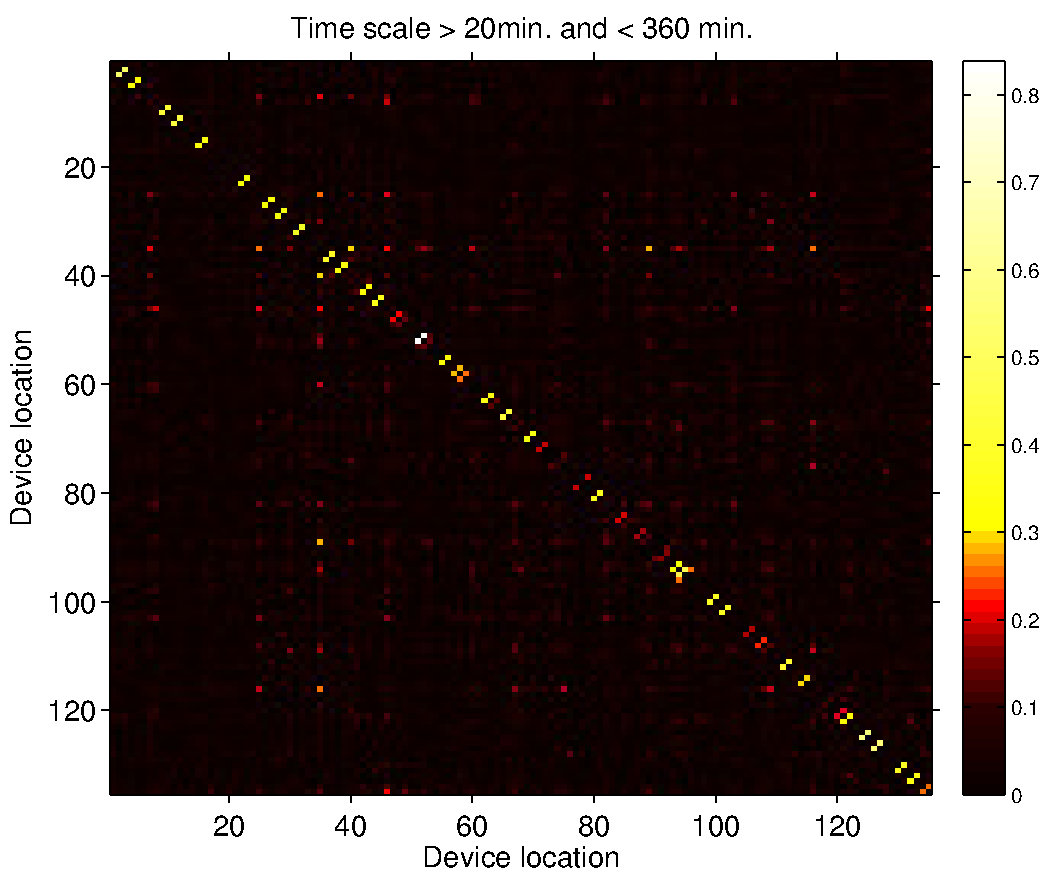
\includegraphics[width=.48\textwidth]{figs/heatMap_2_201106-eps-converted-to.pdf}}\\
\subfloat[Low Frequencies\label{fig:heatmap:low}]{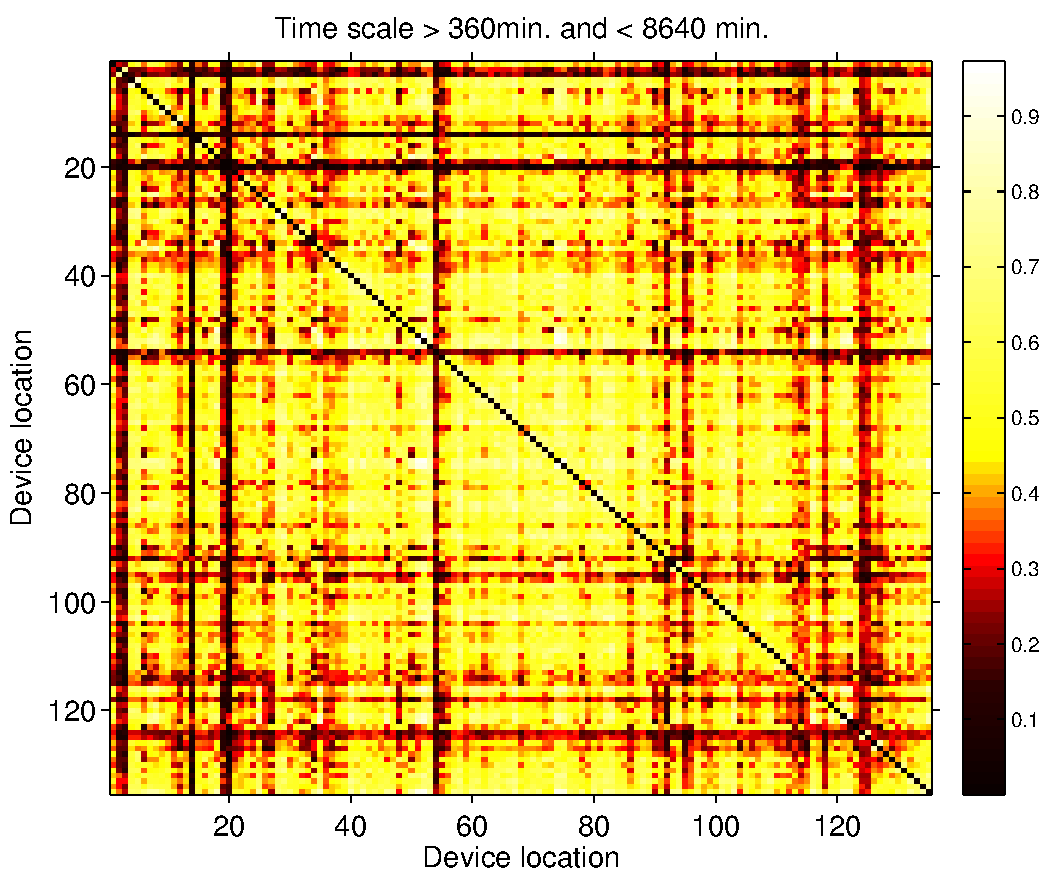
\includegraphics[width=.48\textwidth]{figs/heatMap_3_201106-eps-converted-to.pdf}}\hfill
\subfloat[Residual data\label{fig:heatmap:res}]{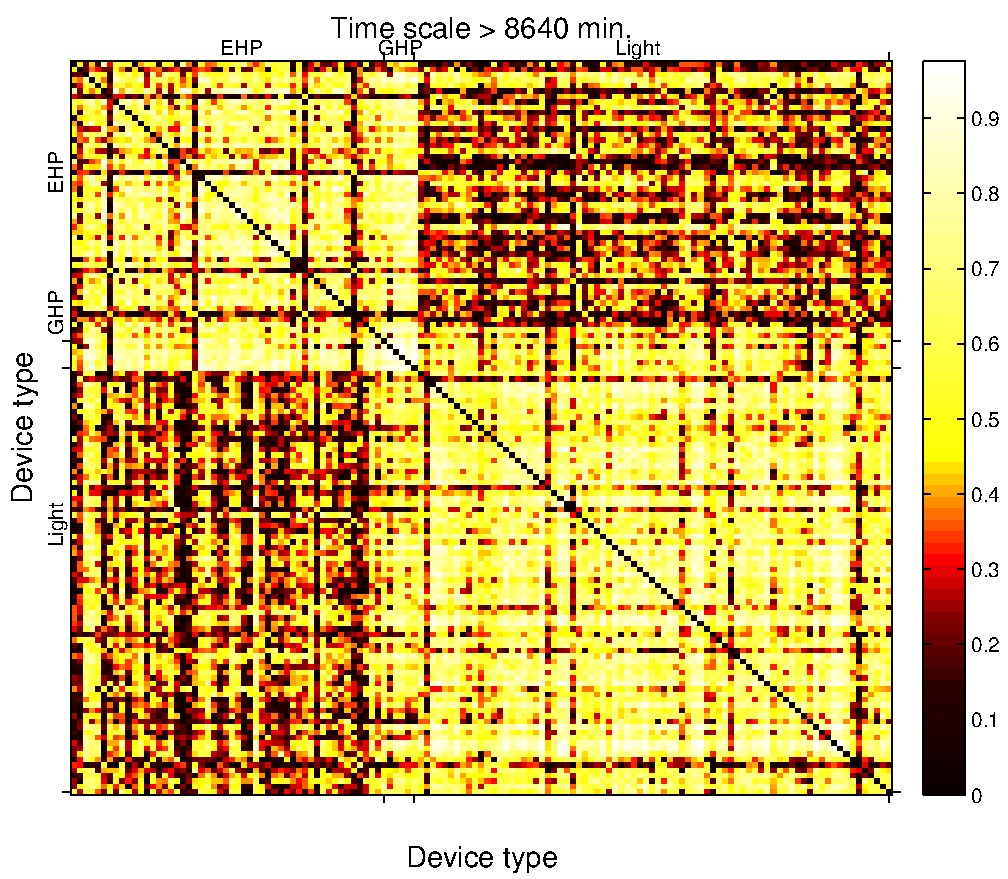
\includegraphics[width=.48\textwidth]{figs/heatMap_4_201106-eps-converted-to.pdf}}
\caption{Reference matrices for the four time scale ranges (the diagonal $x=y$ is colored in black for better reading). The medium frequencies highlight devices that are located next to each other thus intrinsically related. The low frequencies contains the common daily pattern of the data. The residual data permits to visually identify devices of the similar type.}
\label{fig:heatmap}
\end{figure*}

In this section we evaluate SBS on our building traces.  We demonstrate
 the benefits of striping the data by monitoring patterns captured at different time scales.
Then, we thoroughly investigate the alarms reported by SBS.  

\subsection{Device behavior at different time scales}
The Strip and Bind part of SBS is evaluated using the data from Eng. Bldg 2. %, since we can verify how items are being used and use it as ground truth.
This dataset is appropriate to measure SBS's performance, since lighting and HVAC systems serving the same room are usually used 
simultaneously.
Consequently, we analyze this data using SBS and verify that the higher correlations at medium frequencies correspond to devices located in the same room. % and the unwanted data is captured at the other frequencies.

The dataset is split into 10, one-week bins and each bin is processed by SBS.
Using the 10 correlation matrices at each time scale range, SBS uncovers the four reference matrices depicted in 
Figure~\ref{fig:heatmap}.

\paragraph{High frequencies}
In this work the high frequencies correspond to the signals \emph{noise}, 
therefore, we do not expect any useful information from the corresponding matrix (Figure \ref{fig:heatmap:high}).
Indeed, the corresponding reference matrix does not provide any help to determine a device's relative location.
Thus, we emphasize that high frequency data should be ignored for uncovering device relationships (in contrast to \cite{romain:iotapp12}).
Interestingly, we find that the sensors monitoring the lights generate consistent noise. % and could help one to cluster this type of sensor.
  
\paragraph{Medium frequencies}
Our main focus is on the medium frequencies as it is designed to capture the intrinsic device relationships.
Figure \ref{fig:heatmap:med} shows the correlation matrix at medium frequencies.
It is significantly different from the one obtained with the raw signals (Figure \ref{fig:heatmap:raw}): high correlation coefficients are concentrated along the matrix diagonal. 
Since devices serving the same or adjacent rooms are placed nearby in the matrix it validates our hypothesis: \emph{high correlation scores within the medium frequency band shows strong inter-device relationships}.

Considering this reference matrix as an adjacency matrix of a graph, in which the nodes are the devices, we identify the clusters of 
correlated devices using a community mining algorithm~\cite{blondel:unfolding}.
As expected we obtain mainly clusters of only two devices (light and HVAC serving the same room), but we also find clusters that are composed of more devices.
For example a cluster contains 3 HVAC systems serving the three server rooms. Although these server rooms are located on
 different floors, SBS shows a strong correlation between these devices.  Coincidentally, they are managed similarly.
Interestingly, we also observe a couple of clusters that consist of independent devices serving adjacent rooms belonging to the same lab.
The bigger cluster contains 33 devices that are 2 GHP devices and the corresponding lights.
This correlation matrix and the corresponding clusters 
highlight the ability for SBS to identify such hidden inter-device usage relationships.
 
\paragraph{Low frequencies}
Low frequencies capture daily patterns, embedded in all the device traces.  
Figure \ref{fig:heatmap:low} depicts the corresponding reference matrix which is similar to the one of raw signal traces (Figure \ref{fig:heatmap:raw}) 
and it shows no particular structure.% (daily patterns account for the coefficients high values).  
% Since this matrix contains mainly high values, most of the partial signals at low frequencies features similar characteristics (i.e. daily patterns).
These partial signals are discarded as they do not help us in identifying inter-device usage patterns.
 
\paragraph{Residual data}
The residual data shows the weekly trend, which gives us no information about device relationships.
But, surprisingly, by reordering the correlation matrix based on the type of the devices (Figure \ref{fig:heatmap:res}) 
we can visually identify two major clusters.
The first cluster consists of HVAC devices (see EHP and GHP in Figure \ref{fig:heatmap:res}) and the second one contains only lights. 
An in-depth examination of the data reveals that long-term trends are inherent to the device types. 
For example, as the consumption of both the EHP and GHP devices is driven by the building occupancy and the outside temperature, these two types of devices follow the same trend. 
However, the use of light is independent from the outside temperature thus the lighting systems follow a common trend different from the EHP and GHP one.

We conduct the same experiments by splitting the dataset in 70 bins of 1 day long and observe analogous results at high and medium frequencies but not at lower frequencies.  This is because the bins are too short to exhibit daily oscillations and the residual data captures only the daily trend.

% TODO add some info about the reference matrix for the Building 2?










\subsection{Methodological Shortcomings}
Because our analysis is done on historical data, some of the faults found by SBS could not be fully
corroborated.  In order to fully examine the effectiveness of our approach, we must run it in real time and
physically check that the problem is actually occurring.  When a problem is detected
in the historical trace, months after it has occurred, the current state of the building may no longer reflect
what is in the traces.  Some of the anomalies discussed in this section uncover interpretable patterns 
that are difficult to find in practice.  For example, simultaneous heating and cooling is a known, recurring problem
 in buildings, but it is very hard to identify  when it is occurring.  Some of the anomalies we could not interpret
might be interpretable by a building manager, however, we did not consult either building manager for this study.
Therefore, the results of this study do not examine the true/false positive rate exhaustively.

The true/false negative rate is impractical to assess.  It may be examined through synthetic stimulation of
the building via the control system.  However, getting cooperation from a building manager to hand over control of the building
for experimentation in non-trivial.  Therefore, we forgo a full true/false negative analysis in our evaluation.

Because of these challenges, the evaluation of SBS focuses on comparing the output with known fault
signatures.  We examine anomalies, in either building, where the anomaly is easily interpretable but
difficult to find by the building manager.  We forego a comparison of SBS with competing algorithms because
 related algorithms require detailed knowledge of the building, \emph{a priori}.  The advantage of SBS is that it 
requires no such information to provide immediate value.